%======================================================================
\section{Introduction}\label{sec:intro}
%======================================================================
Electric vehicles (EVs) parked at workplaces form one of the largest controllable electricity loads that buildings and distribution networks will host. Cars stay plugged in for most of the working day but need only a few hours at Level-2 power to recover their daily energy, so the timing of their demand is, in principle, highly flexible \cite{Lee2019ACNData,Schuller2015Flex,Develder2016Flex}. Whether this flexibility is realised determines the grid impact of electrified commuting: uncoordinated charging raises local peaks even at low adoption \cite{Muratori2018Uncoordinated,ClementNyns2010,Gong2012Transformer}, the operation of charging infrastructure is a first-order lever at scale \cite{Powell2022Infrastructure,Crozier2020SmartCharging,Mangipinto2022Europe}, and aggregators increasingly seek to trade EV flexibility in electricity markets \cite{Chemudupaty2025Intraday,Chemudupaty2025SpotMarkets}. At the site level, the concentration of morning arrivals that creates flexibility also creates a sharp peak, which commercial tariffs price through demand charges per kilowatt of the highest demand in the billing month \cite{Lee2020Pricing}. Demand charges are thus the signal through which local peak reduction, the most direct distribution-level benefit of smart charging, reaches the site operator.

Smart charging can flatten the site load because each session has laxity: the time a vehicle is plugged in usually far exceeds the time needed to deliver its energy \cite{Lee2019ACNData,Nakahira2017sLLF}. Exploiting laxity online, however, requires knowing when each vehicle will leave and how much energy it needs. Deployed systems such as the Adaptive Charging Network (ACN) ask drivers to declare both quantities through a mobile application at plug-in \cite{Lee2021ACN}. The ACN-Data study showed that these declarations are a poor predictor of realised behaviour, worse than simple statistical predictors trained on past sessions \cite{Lee2019ACNData}. A scheduler that takes declarations at face value can therefore plan to finish charging after a car has already left, or reserve peak capacity for energy that will never be requested.

Demand charges make this uncertainty costly in a specific way. Because the demand charge is levied on the monthly maximum, a peak created by one poorly planned afternoon is paid for the whole month; conversely, once a peak has been set, any later load below it carries no additional demand charge. Lee, Pang and Low \cite{Lee2020Pricing} exploited this structure in an online model predictive controller (MPC) evaluated on ACN-Data, but, like most online schedulers, their controller trusts the declared departure time and energy. Competitive-ratio methods for online peak minimisation provide worst-case guarantees against arrival uncertainty \cite{Zhao2017RobustOnline}, but they do not use the large empirical record of declaration errors that open datasets now provide.

How much of the theoretical flexibility of workplace charging can actually be realised is therefore an open energy-system question. It matters beyond the site: a workplace fleet whose peak can be reliably held below a limit is a resource that a distribution operator, an aggregator or a virtual power plant can plan with. Parking duration and connected capacity bound flexibility from above \cite{Develder2016Flex,Schuller2015Flex}, but an online controller can only use the flexibility it knows about, and what it knows comes largely from user information of uncertain quality \cite{Lee2019ACNData,Kreft2024Predictability}. This paper asks: how much of the technical flexibility of workplace EV charging can be reliably converted into grid-usable flexibility when user information is imperfect, and how do tariff signals determine whether that flexibility is activated? We make five contributions.
\begin{enumerate}
\item We build on the demand-charge-aware MPC of Lee, Pang and Low \cite{Lee2020Pricing}, writing it as a peak-state receding-horizon linear program in which the month-to-date peak is a state, so that only increments above it are priced. The controller form is not our contribution; what is new is that we derive a data-driven robust counterpart for declaration errors that is exactly the nominal problem with shifted deadlines and scaled energy targets. A PV-aware variant prices grid import rather than EV load.
\item We evaluate uncontrolled charging, earliest-deadline-first (EDF), least-laxity-first (LLF), nominal, robust and PV-aware MPC and a hindsight optimum by event-driven replay of \JPLtestN{} (JPL) and \CALtestN{} (Caltech) real sessions from July to December 2019, under the SCE TOU-EV-4 tariff in force during the data period \cite{SCETOUEV4}, with uncertainty sets calibrated strictly on preceding data.
\item We report a negative result and its diagnosis. Acting on declarations leaves about one vehicle in eight short of its energy, and calibrated robustness does not repair this at any protection level, because declared energy is biased upwards while departure errors are wide.
\item We quantify grid-usable flexibility: peak reduction, load factor, ramps and shifted energy; transformer loading and the service deliverable within transformer ratings; PV self-consumption under PV-unaware and PV-aware control; and how the demand-charge level and energy-price structure determine whether peak reduction is delivered.
\item We propose a peak-state top-up rule that re-uses capacity already billed in the month, restoring energy service to above 99\% without creating a new peak. We validate it in simulation on held-out 2021 sessions that played no part in its design (97--99\% served), under altered capacity, tariff, calibration and penalty settings, and with demand up to 23\% above the historical record (96--99.5\% served). The analysis builds only on openly licensed data \cite{ACNDataset,Yeh2023SustainGym}.
\end{enumerate}

Section~\ref{sec:lit} positions the work. Section~\ref{sec:data} describes the data and tariff, Section~\ref{sec:method} the models, and Section~\ref{sec:design} the experimental design. Results are reported in Section~\ref{sec:results} and discussed in Section~\ref{sec:discussion}; Section~\ref{sec:conclusion} concludes.

%======================================================================
\section{Related work and research gap}\label{sec:lit}
%======================================================================
\subsection{EV charging flexibility and grid impacts}
Charging strategy, rather than the number of EVs alone, determines grid impact. Uncoordinated charging stresses voltages and transformers \cite{ClementNyns2010,Putrus2009Impact,Gong2012Transformer}, and clustered adoption amplifies local peaks \cite{Muratori2018Uncoordinated,Fischer2019Residential,KamanaWilliams2024Peak}. Controlled charging lowers peak residual load and system cost \cite{Hanemann2017Strategies,Schill2015Germany,Mangipinto2022Europe,Crozier2020SmartCharging,Heuberger2020EVolution,Strobel2022Regional}, reduces renewable curtailment \cite{Szinai2020GridCosts,Denholm2013PV} and supports generation adequacy, also through vehicle-to-grid \cite{Kempton2005Fundamentals,Kempton2005Implementation,Frank2025Germany,Lauvergne2022Adequacy}; see \cite{Richardson2013Review,Li2026UltraFast} for reviews. We consider unidirectional workplace charging, which the studied sites support. Offline formulations such as valley filling \cite{Chen2014ValleyFilling}, network-constrained scheduling \cite{deHoog2015Network} and aggregator optimisation \cite{Rivera2017Aggregators} value this flexibility when session parameters are known.

\subsection{Online control under behavioural uncertainty}
Online methods act without knowing future departures and energy needs: least-laxity-first variants \cite{Nakahira2017sLLF}, predictive scheduling under user uncertainty \cite{Wang2016Predictive}, building energy management with workplace charging \cite{Wu2017Office}, deadline extension with on-site solar \cite{Ardakanian2014Deadlines,Lee2016SharedSolar}, simulation studies \cite{Ramanujam2017Impact} and two-layer predictive control on ACN-Data \cite{Ahmad2023TwoLayer}. Open data make them comparable: ACN-Data \cite{Lee2019ACNData}, the ACN-Sim simulator \cite{Lee2021ACNSim}, the deployed ACN \cite{Lee2021ACN}, SustainGym benchmarks \cite{Yeh2023SustainGym} and other public datasets and generators \cite{Flammini2019Stats,Lucas2018Indicators,GaeteMorales2021emobpy}. Energy-system studies treat EV charging as a flexibility resource whose value depends on behaviour, quantifying the effect of user preferences on spot- and intraday-market value \cite{Chemudupaty2025SpotMarkets,Chemudupaty2025Intraday}, heterogeneous predictability \cite{Kreft2024Predictability} and trip-chain flexibility \cite{Tang2025TripChain}, usually with behaviour as a stochastic input. Robust optimisation protects constraints against an uncertainty set \cite{Soyster1973}, with budgeted \cite{Bertsimas2004Price} or data-driven \cite{Bertsimas2018DataDriven,Esfahani2018Wasserstein} sets controlling conservatism \cite{Gorissen2015Guide,Mayne2014MPC}.

\subsection{Research gap and contribution}
Lee, Pang and Low \cite{Lee2020Pricing} are closest to this paper. They proposed session-level pricing of energy, demand-charge and congestion costs, and an online MPC whose cost on ACN-Data was within about ten per cent of the offline optimum, with declared energy and departure taken as given. Demand-charge-aware MPC on ACN-Data is therefore established, and we do not claim it as new. Zhao, Lin and Chen \cite{Zhao2017RobustOnline} give worst-case guarantees for online peak minimisation that are not calibrated to observed declaration errors. Table~\ref{tab:lit} compares this study with the most closely related work, and Table~\ref{tab:contrib} maps the remaining gaps to its contributions. No previous study measures how much of the grid flexibility of workplace charging is realisable when drivers' information is imperfect, tests whether robustness calibrated to that information helps, or relates the outcome to the tariff that remunerates flexibility.

\begin{table}[!htbp]
\centering
\caption{Comparison of this study with closely related literature (chronological order).}
\label{tab:lit}
\scriptsize
\setlength{\tabcolsep}{2.5pt}
\renewcommand{\arraystretch}{1.12}
\begin{tabular*}{\textwidth}{@{\extracolsep{\fill}}*{6}{>{\raggedright\arraybackslash}p{0.148\textwidth}}@{}}
\hline
Study & Focus and method & User information & Tariff and grid outcome & Data and validation & Gap left open \\
\hline
Nakahira et al.\ (2017) \cite{Nakahira2017sLLF} & Online smoothed least-laxity-first & Declared values used as given & Capacity-feasible service; no tariff signal & Real sessions & No cost, demand charge or grid-flexibility metrics \\
Zhao, Lin \& Chen (2017) \cite{Zhao2017RobustOnline} & Online peak minimisation (competitive ratio) & Worst-case (adversarial) & Peak only & No real sessions & Guarantees not calibrated to observed errors \\
Lee, Li \& Low (2019) \cite{Lee2019ACNData} & ACN-Data release and analysis & Predicted (Gaussian mixture) & Demand charge used for sizing only & Real sessions & No online control under demand charges \\
Lee, Pang \& Low (2020) \cite{Lee2020Pricing} & Session pricing; demand-charge-aware MPC & Declarations taken as given & Bill including demand charge & ACN-Data & Service loss from declaration errors unmeasured; no robustness or grid metrics \\
Lee et al.\ (2021) \cite{Lee2021ACNSim} & Open-source simulator (ACN-Sim) & Declared values, no error model & Demand charge optional & ACN-Data; open code & A platform, not an analysis of information quality \\
Ahmad et al.\ (2023) \cite{Ahmad2023TwoLayer} & Two-layer predictive control & Load predicted without departure input & TOU energy cost; no demand charge & Caltech ACN-Data & No peak state or grid-flexibility metrics \\
Kreft et al.\ (2024) \cite{Kreft2024Predictability} & Prediction of session duration and energy & Predictability varies strongly across users & Not evaluated in control & 267 residential EVs & Prediction only; no control or tariff \\
Chemudupaty et al.\ (2025) \cite{Chemudupaty2025SpotMarkets} & Scenario-based robust optimisation & User preferences (min.\ SOC, plug-in frequency) & Day-ahead and intraday procurement cost & German markets, 2022--2023 & Market value, not site peak under measured declaration errors \\
\textbf{This study} & Peak-state MPC, calibrated robust counterpart, top-up, PV-aware variant & Empirical declaration errors, calibrated out of sample & Bill, peak, PAR, ramps, transformer loading, PV use, tariff designs & 13,623 sessions; held-out 2021; open code & -- \\
\hline
\end{tabular*}
\end{table}

\begin{table}[!htbp]
\centering
\caption{Research gaps, methodological response and contributions of this study.}
\label{tab:contrib}
\scriptsize
\setlength{\tabcolsep}{2.5pt}
\renewcommand{\arraystretch}{1.12}
\begin{tabular*}{\textwidth}{@{\extracolsep{\fill}}>{\raggedright\arraybackslash}p{0.2\textwidth}>{\raggedright\arraybackslash}p{0.24\textwidth}>{\raggedright\arraybackslash}p{0.2\textwidth}>{\raggedright\arraybackslash}p{0.25\textwidth}@{}}
\hline
Research gap & Methodological response & Novelty & Key finding (Section) \\
\hline
G1. Effect of real declaration errors on realisable flexibility is unquantified & Error distributions of claimed sessions; rolling out-of-sample calibration; event-driven replay & First measurement under a monthly demand-charge state & Peak halved, but one vehicle in eight left short of its energy (\ref{sec:res:diag}) \\
G2. Robustness never calibrated to observed errors & Exact data-calibrated robust counterpart (earlier deadlines, scaled targets) & Robustness shown to fail at every protection level, with diagnosis & No protection level beats nominal MPC; fragile under 2021 behavioural drift (\ref{sec:res:robust}, \ref{sec:res:heldout}) \\
G3. No recourse to realised behaviour under demand charges & Peak-state top-up that fills capacity already billed in the month & Recourse step that cannot raise a billed peak & Over 99\% of historical energy served at the same peak; 97--99\% on held-out data; 96--99.5\% with higher demand (\ref{sec:res:topup}--\ref{sec:res:topuprob}) \\
G4. Site control rarely expressed as grid-deliverable flexibility, or related to tariff design & Flexibility metrics, transformer limits, PV-aware control, tariff sweep and archetypes & Joint service--cost--grid evaluation & Half-rated transformer kept within rating at 99\% service; presence of a demand charge decides peak reduction (\ref{sec:res:flex}, \ref{sec:res:pvaware}--\ref{sec:res:arch}) \\
\hline
\end{tabular*}
\end{table}

%======================================================================
\section{Data and tariff}\label{sec:data}
%======================================================================
\subsection{Sessions}
ACN-Data is an open dataset of workplace charging sessions collected by the Adaptive Charging Networks at Caltech and at NASA's Jet Propulsion Laboratory (JPL) \cite{Lee2019ACNData,ACNDataset}. JPL access is restricted to employees and represents workplace charging; the Caltech garage is open to the public and mixes workplace and public use \cite{Lee2019ACNData}. We use the session extracts for 1 May--31 December 2019 that SustainGym v0.1.7 redistributes under a CC-BY-4.0 licence \cite{Yeh2023SustainGym}; SustainGym obtained them through the official ACN-Data API and kept the first user input of every claimed session. The period lies after Caltech's switch to paid charging on 1 November 2018 \cite{Lee2019ACNData} and before the 2020 pandemic, so neither break falls inside a training or test window. For out-of-sample validation we also use the SustainGym extract for 1 May--31 August 2021, which was not used at any stage of model design; its Caltech portion contains 423 sessions with implied average power above 20\,kW (the site's DC fast charger), which the power filter removes. File checksums are provided with the code.

Each session records the plug-in time, the disconnect time and the delivered energy. For \emph{claimed} sessions the driver also declared, at plug-in, an estimated departure time and a requested energy. For unclaimed sessions SustainGym fills these two fields with the realised values; because that would leak future information into an online controller, we discard them and let a calibrated predictor supply the declaration (Section~\ref{sec:calib}). The extract does not contain the time at which charging stopped, so the maximum charging rate of a session is set to $\bar r_i=\max(6.6\,\text{kW},\,e_i/(\text{duration}_i))$, which guarantees that the observed energy is deliverable. Table~\ref{tab:data} summarises the data; the filtering flow (Table~S1) and daily energy with weekday arrival and departure profiles (Fig.~S1) are given in the Supplementary Material.

\begin{table}[!htbp]
\centering
\caption{ACN-Data sessions used in this study (1 May--31 December 2019).}
\label{tab:data}
\footnotesize
\setlength{\tabcolsep}{1.5pt}
\begin{tabular*}{\textwidth}{@{\extracolsep{\fill}}lrrrrrrr@{}}
\hline
Site & \makecell[c]{Raw\\sessions} & \makecell[c]{Retained\\sessions} & \makecell[c]{Energy\\(MWh)} & \makecell[c]{Claimed\\(\%)} & \makecell[c]{Median\\stay (h)} & \makecell[c]{Median\\kWh} & \makecell[c]{Weekday\\(\%)} \\
\hline
JPL & 11,830 & 11,823 & 171.8 & 96.8 & 8.30 & 11.60 & 97.1 \\
Caltech & 6,704 & 6,659 & 57.4 & 84.3 & 5.73 & 5.93 & 90.6 \\
\hline
\end{tabular*}
\end{table}


\subsection{Declaration errors}
Fig.~\ref{fig:errors} shows the empirical distribution of the two declaration errors for claimed sessions: the departure error $\Delta d_i=d_i-\hat d_i$ (positive when the driver stays longer than declared) and the energy ratio $\rho_i=e_i/\hat e_i$. \ErrorSentence

\begin{figure}[!htbp]
\centering
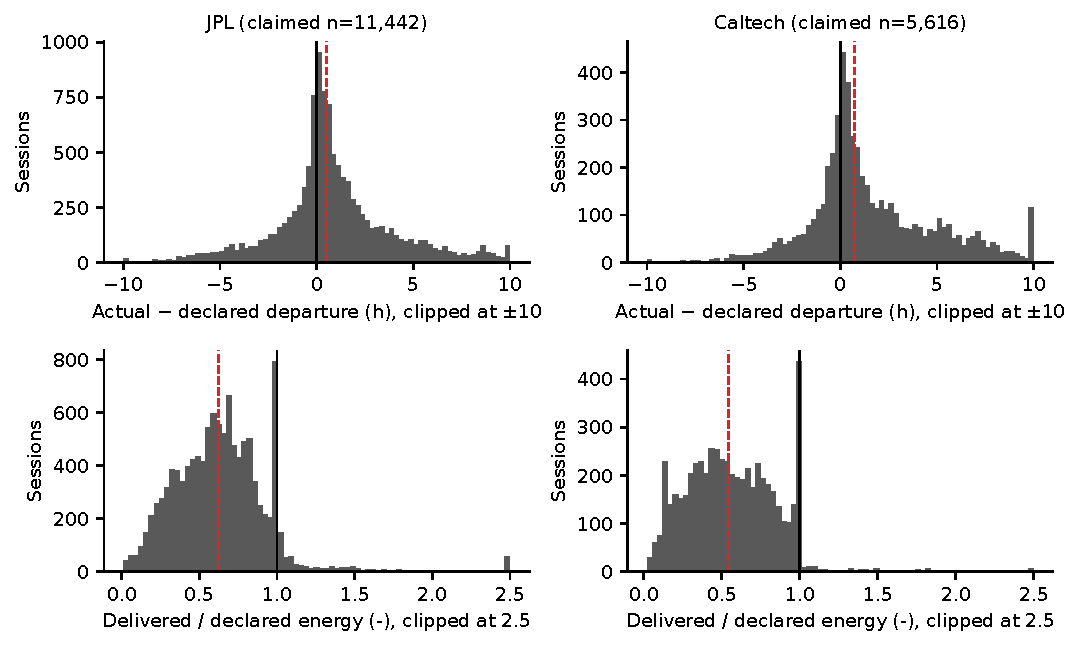
\includegraphics[width=0.7\textwidth]{figures/Fig3_declaration_errors.pdf}
\caption{Declaration errors of claimed sessions. Top: actual minus declared departure time. Bottom: delivered over declared energy. Dashed lines mark medians.}
\label{fig:errors}
\end{figure}

\subsection{Tariff}\label{sec:tariff}
We bill every policy under SCE Schedule TOU-EV-4 effective 1 March 2019 \cite{SCETOUEV4}, the tariff contemporaneous with the data, using the rate values encoded in the ACN research portal \cite{Lee2021ACNSim}. It combines time-of-use energy prices with a demand charge of 15.51\,USD per kW of monthly maximum demand. SCE's later commercial EV schedules carried a period without demand charges \cite{CPUCEVRates}, which would remove the problem studied here, so the demand-charge level is instead varied in the sensitivity analysis. General-service schedules for EV load on a shared building meter combine a facilities-related and a time-related demand charge \cite{SCETOUGS2}; our formulation includes both terms, and the time-related term is zero in the base case. In summer (June--September) weekday energy costs 0.05623\,USD/kWh at 23--08\,h, 0.0925\,USD/kWh at 08--12\,h and 18--23\,h, and 0.26668\,USD/kWh at 12--18\,h; the winter prices for the same periods are 0.06087, 0.07492 and 0.0869\,USD/kWh, and weekends are charged at the off-peak price (Table~S2 of the Supplementary Material). Holidays and customer charges are not modelled, and the EV load is assumed to be separately metered.


%======================================================================
\section{Methodology}\label{sec:method}
%======================================================================
Figure~\ref{fig:framework} summarises the framework.

\begin{figure}[!htbp]
\centering
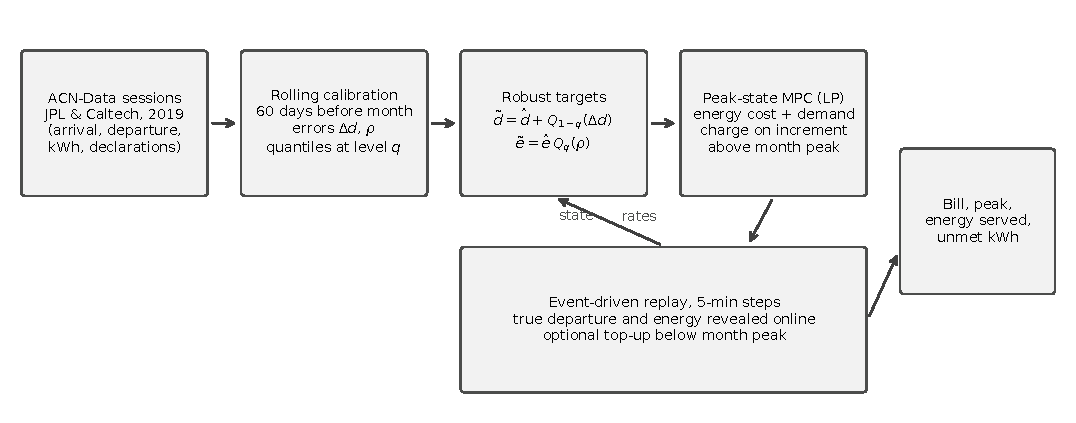
\includegraphics[width=0.7\textwidth]{figures/Fig1_framework.pdf}
\caption{Framework: rolling calibration of declaration errors, robust targets, peak-state MPC, and event-driven replay against realised sessions.}
\label{fig:framework}
\end{figure}

\subsection{Notation}
Time is discretised into periods $t\in\mathcal T=\{0,\dots,T-1\}$ of length $\Delta=5$\,min. Session $i\in\mathcal V$ arrives at $a_i$, departs at $d_i$ and accepts energy $e_i$ (kWh) at up to $\bar r_i$ (kW). At plug-in the controller observes a declaration $(\hat d_i,\hat e_i)$. The site capacity is $C$, energy prices are $c_t$ (USD/kWh), $\lambda^{F}$ is the facilities-related demand charge on the monthly maximum over all periods and $\lambda^{T}$ the time-related charge on the maximum over the set $\mathcal T^{\text{on}}$ of on-peak periods. The decision $r_{it}\ge0$ is the charging rate of session $i$ in period $t$.

\subsection{Hindsight benchmark}
With perfect knowledge of every $(a_i,d_i,e_i)$ in the month, the minimum bill solves the linear program
\begin{align}
\min_{r,s,P^F,P^T}\;& \sum_{t\in\mathcal T}\sum_{i\in\mathcal V} c_t\,\Delta\, r_{it} \;+\; \lambda^F P^F \;+\; \lambda^T P^T \;+\; M\sum_{i\in\mathcal V} s_i \label{eq:obj}\\
\text{s.t.}\;& \Delta\!\!\sum_{t=a_i}^{d_i-1}\! r_{it} + s_i \ge e_i,\qquad \Delta\!\!\sum_{t=a_i}^{d_i-1}\! r_{it}\le e_i, && i\in\mathcal V \label{eq:energy}\\
& 0\le r_{it}\le \bar r_i \;\;(a_i\le t<d_i),\qquad r_{it}=0\;\;\text{otherwise}, && i\in\mathcal V \label{eq:rate}\\
& \textstyle\sum_{i} r_{it}\le C, \qquad \sum_{i} r_{it}\le P^F, && t\in\mathcal T \label{eq:cap}\\
& \textstyle\sum_{i} r_{it}\le P^T, && t\in\mathcal T^{\text{on}} \label{eq:peakon}\\
& 0\le s_i\le e_i . \label{eq:slack}
\end{align}
The slack $s_i$ is undelivered energy penalised at $M$ (5\,USD/kWh in the base case; varied in Section~\ref{sec:sens}). The feasible set follows the ACN scheduling formulation \cite{Lee2019ACNData,Lee2021ACN}; the objective adds the demand charge as in \cite{Lee2020Pricing}.

\subsection{Peak-state receding-horizon control}
Online, at period $\tau$ the controller knows only the sessions present, their declarations, the energy already delivered $\delta_i(\tau)$, and the realised month-to-date peaks $\hat P^F(\tau)=\max_{t<\tau}\sum_i r_{it}$ and $\hat P^T(\tau)$ (the latter over on-peak periods). It solves \eqref{eq:obj}--\eqref{eq:slack} over the remaining horizon with three changes: (i) the window of session $i$ ends at its planning deadline rather than at its unknown departure, (ii) the energy target is the planning target minus $\delta_i(\tau)$, and (iii) the peak variables are bounded below by the realised peaks,
\begin{equation}
P^F\ge \hat P^F(\tau),\qquad P^T\ge \hat P^T(\tau). \label{eq:peakstate}
\end{equation}
Constraint~\eqref{eq:peakstate} makes the demand-charge term price only the increment $[P^F-\hat P^F(\tau)]^+$: capacity already paid for this month is free, which is the structural property of monthly demand charges that the controller must exploit. The LP is re-solved at every arrival, departure or completion event and at least every 15\,min; between solves the stored plan is applied. A vanishing tie-breaking term $\epsilon\sum_{i,t}(t-\tau)r_{it}$ favours earlier charging among cost-equivalent schedules, as in the deployed ACN \cite{Lee2019ACNData}. Following standard receding-horizon practice \cite{Mayne2014MPC}, only the first-period rates are implemented.

\subsection{Data-calibrated robust counterpart}\label{sec:robust}
Let $\mathcal U_i=[\underline{\Delta d},\overline{\Delta d}]\times[\underline\rho,\overline\rho]$ be a box of plausible declaration errors, so the true departure is $\hat d_i+\Delta d$ and the true energy $\rho\,\hat e_i$ for some $(\Delta d,\rho)\in\mathcal U_i$. A plan is robust for session $i$ if it delivers the required energy before departure for every realisation, i.e.
\begin{equation}
\Delta\!\!\sum_{t=\tau}^{\hat d_i+\Delta d-1}\! r_{it} \;\ge\; \rho\,\hat e_i-\delta_i(\tau)\qquad \forall(\Delta d,\rho)\in\mathcal U_i . \label{eq:robust}
\end{equation}
The left-hand side is non-decreasing in $\Delta d$ because $r_{it}\ge0$, and the right-hand side is increasing in $\rho$. The worst case is therefore attained at the corner $(\underline{\Delta d},\overline\rho)$ and \eqref{eq:robust} is equivalent to the single linear constraint
\begin{equation}
\Delta\!\!\sum_{t=\tau}^{\tilde d_i-1}\! r_{it} \ge \tilde e_i-\delta_i(\tau),\qquad \tilde d_i=\hat d_i+\underline{\Delta d},\quad \tilde e_i=\overline\rho\,\hat e_i . \label{eq:rc}
\end{equation}
This is Soyster's result for column-wise uncertainty \cite{Soyster1973} specialised to the EV constraint structure: the robust controller is the nominal controller with an earlier deadline and a scaled energy target, and it has exactly the same size. Because every constraint involves one session only, a cardinality budget across sessions \cite{Bertsimas2004Price} would not reduce conservatism for constraint-wise protection; conservatism is instead controlled by the size of the box.

\subsection{Rolling calibration}\label{sec:calib}
For a protection level $q\in(0,1)$ we set $\underline{\Delta d}=Q_{1-q}(\Delta d)$ and $\overline\rho=Q_q(\rho)$, the empirical quantiles of the errors observed in the 60 days before the test month, in the spirit of data-driven uncertainty sets \cite{Bertsimas2018DataDriven}. Claimed and unclaimed sessions are calibrated separately. For unclaimed sessions the declaration is a population prediction, the median stay and median energy of unclaimed training sessions with the same weekday flag and three-hour arrival bucket, and its errors are calibrated in the same way. The nominal controller corresponds to $(\underline{\Delta d},\overline\rho)=(0,1)$; $q=0.5$ gives a median-debiased controller, and $q=0.7$ and $0.9$ progressively more conservative ones. Energy delivered never exceeds the true $e_i$: when a vehicle is full its current drops to zero and the controller removes it, as a real system observes.

\subsection{Peak-state top-up}\label{sec:topup}
The robust counterpart can only move targets; it cannot deliver energy that the declarations do not ask for. The top-up rule exploits the same peak-state property as \eqref{eq:peakstate}, but after the LP has been solved. In each period, let $\bar P(\tau)=\min\{\hat P^F(\tau),C\}$, further limited by $\hat P^T(\tau)$ in on-peak periods when $\lambda^T>0$. Any headroom $\bar P(\tau)-\sum_i r_{i\tau}$ is then allocated to vehicles that still accept current, in order of declared departure, up to each vehicle's $\bar r_i$. By construction the top-up never raises a billed peak, so its only cost is the energy price of the additional kWh. We disclose that this rule was designed after, and because of, the diagnosis in Section~\ref{sec:res:diag} on the 2019 test months. To test it out of sample, we apply every policy unchanged to held-out 2021 sessions (Section~\ref{sec:res:heldout}) and under altered capacity, tariff, calibration and penalty settings (Section~\ref{sec:res:topuprob}). Both are simulation validations on recorded sessions, not a field deployment: drivers did not experience the top-up schedules, so behavioural responses to them are not captured.

\subsection{Grid-flexibility and solar-coincidence metrics}\label{sec:metrics}
Besides cost and service, we evaluate each realised monthly load profile $L_t$ with metrics of realised demand flexibility: peak reduction relative to uncontrolled charging, $\max_t L^{\text{unc}}_t-\max_t L_t$; the load factor $\bar L/\max_t L_t$ and its inverse, the peak-to-average ratio (PAR); the maximum change between consecutive 15-min averages (ramp); shifted energy, $\Delta\sum_t[L^{\text{unc}}_t-L_t]^+$; and the share of energy delivered in the weekday 12--18\,h on-peak block.
For the baseline, PV-unaware controllers, solar coincidence tests whether peak-state scheduling moves charging towards or away from solar hours. We build a clear-sky irradiance profile for each site with the Ineichen model in pvlib \cite{Holmgren2018pvlib,Anderson2023pvlib} and treat it as the output shape of a horizontal PV array. The array is sized so that its monthly energy equals the monthly EV demand ("energy-neutral"; a half-size array is a sensitivity). PV self-sufficiency is $\sum_t\min(L_t,PV_t)/\sum_t L_t$ and PV utilisation $\sum_t\min(L_t,PV_t)/\sum_t PV_t$.

\subsection{PV-aware peak-state control}\label{sec:pvaware}
To test whether the controller can exploit on-site generation rather than merely coincide with it, we add a behind-the-meter PV profile $PV_t$ (kW) and introduce the grid import $g_t\ge 0$ as a decision variable. The PV-aware controller solves \eqref{eq:obj}--\eqref{eq:slack} with the energy cost and both peaks applied to import instead of to EV load:
\begin{align}
g_t &\ge \textstyle\sum_i r_{it}-PV_t, \qquad g_t\le P^F\quad (t\in\mathcal T), \qquad g_t\le P^T\quad (t\in\mathcal T^{\text{on}}), \label{eq:pvaware}\\
&\text{with energy cost } \textstyle\sum_t c_t\,\Delta\, g_t \text{ replacing } \sum_{t,i} c_t\,\Delta\, r_{it} \text{ in \eqref{eq:obj}}. \nonumber
\end{align}
Surplus PV is assumed to be curtailed without export credit, so the controller is rewarded only for self-consumption. The top-up ceiling becomes $\min\{\hat P^F(\tau)+PV_\tau,\,C\}$, so top-up also absorbs surplus PV without raising the billed import peak. The PV profile is the energy-neutral clear-sky profile of Section~\ref{sec:metrics}. All policies, including PV-unaware ones, are billed on metered import in this scenario, so their costs are directly comparable.

\subsection{Transformer hosting limits}\label{sec:xfmr}
The site peak is only a proxy for distribution-network impact. To make the network dimension explicit, we represent the EV supply transformer as a hard import limit $\bar S$ and evaluate two hosting scenarios, in which the transformer rating is 50\% and 35\% of the six-month mean uncontrolled peak (148\,kW and 104\,kW at JPL; 52\,kW and 37\,kW at Caltech). They represent fleets on an existing transformer not sized for uncontrolled charging. Uncontrolled charging ignores the limit, and we report its maximum loading (per unit of rating), overload duration and overload energy. Controlled policies receive $\bar S$ as their capacity $C$; for them we report the energy service they can still deliver within the limit, which is the flexibility that is actually deliverable to the network operator.

\subsection{Tariff archetypes}\label{sec:archetypes}
To test transferability beyond the historical SCE schedule, we keep the TOU-EV-4 demand charge and evaluate two stylised archetypes: an \emph{evening-peak TOU}, with the on-peak block moved to 16--21\,h on weekdays as in recent tariffs of solar-rich systems, and a \emph{flat energy price} equal to the monthly time-weighted TOU-EV-4 mean, representing demand-charge tariffs without time-of-use energy prices. They are not actual tariffs; they isolate how the energy-price structure interacts with the demand charge.

%======================================================================
\section{Experimental design}\label{sec:design}
%======================================================================
\subsection{Policies}
We compare seven policy families on identical sessions: (1) \emph{Uncontrolled}, every vehicle charges at $\bar r_i$ from plug-in until full, without a capacity limit; (2) \emph{EDF}, earliest declared deadline first, and (3) \emph{LLF}, least declared laxity first, both allocating $\bar r_i$ in priority order up to $C$; (4) \emph{Nominal MPC}, the peak-state controller using declarations as given, which follows the design of \cite{Lee2020Pricing}; (5) \emph{Robust MPC}$(q)$ with $q\in\{0.5,0.7,0.9\}$; (6) \emph{MPC + top-up}, nominal and robust MPC ($q\in\{0.7,0.9\}$) with the rule of Section~\ref{sec:topup}; and (7) the \emph{hindsight optimum} of \eqref{eq:obj}--\eqref{eq:slack}, a lower bound on the penalised cost of any capacity-feasible policy. In the PV scenario, MPC + top-up and the hindsight optimum are also run in their PV-aware form (Section~\ref{sec:pvaware}).

\subsection{Replay and metrics}
Each test month (July--December 2019) is replayed at 5-min resolution. Sessions are assigned to the month of arrival, and the site capacities are 195\,kW (JPL) and 150\,kW (Caltech) \cite{Lee2019ACNData}. We report the monthly bill (energy plus demand charges on realised load), the monthly peak, the share of demanded energy served (demand being the energy each vehicle actually received in the recorded session, see below), the share of vehicles fully served (within 0.05\,kWh), and the bill gap to the hindsight optimum. LPs are solved with HiGHS \cite{Huangfu2018HiGHS} through SciPy and its Python interface \cite{Virtanen2020SciPy}. Because the ACN was itself a managed system, the recorded delivered energy may fall short of what some drivers would have taken without control; all service figures in this paper are therefore measured against historically delivered energy, not against unconstrained charging needs. Software integrity checks on synthetic data confirm that no controlled policy exceeds capacity, that delivered energy never exceeds demanded energy, and that the hindsight optimum lower-bounds the penalised cost of every controlled policy.

\subsection{Sensitivity analysis}\label{sec:sens}
For August and November 2019 we vary the demand charge (0 and twice the tariff value), the calibration window (30 and 90 days) and the shortfall penalty ($M=20$\,USD/kWh) for nominal MPC, robust MPC at $q=0.9$ and, where the objective changes, the hindsight optimum. The top-up rule is tested separately under these and further settings (Section~\ref{sec:res:topuprob}). Separately, a tariff-design sweep evaluates uncontrolled charging, MPC + top-up and the hindsight optimum for demand charges of 0, 5, 10, 15.51, 20 and 31.02\,USD/kW-month in the same two months. The PV-aware scenario covers all six test months; the transformer scenarios and tariff archetypes use August and November 2019.
